\documentclass{article}

\usepackage[a4paper]{geometry} % Seitenlayout, Standard: A4 Portrait
\usepackage{polyglossia}
\usepackage{graphicx}
\usepackage{tcolorbox}
\usepackage{tikz}
\usepackage{tikz-3dplot}
\usepackage[utf8]{inputenc}% bei einer aktuellen TeX-Distribution nicht nötig
\usepackage[T1]{fontenc}
\usepackage{lmodern}
\usepackage{array}
\usepackage{xbox}
\usepackage{longtable}
\usepackage{graphicx}
\usepackage{caption}[2008/04/01]
\usepackage{wrapfig}

\catcode`\ß=\active\defß{\ss} % necessary not to have "StrauSS" for "Strauß"

\setdefaultlanguage[spelling=new]{german}
\geometry{left=2cm,right=2cm,top=1.4cm,bottom=2cm}

\graphicspath{{images/}}

\usetikzlibrary{
	matrix,
	positioning,
	arrows.meta,
	backgrounds,
	angles,
	quotes,
	babel,
	calc
}


\title{
	\bf\sf\Huge Roomscanner\\[-5mm]
	\Large Dokumentation
}
\author{
Kolja Lingsma
\and
Maxi Bornhofen\thanks{Author der Dokumentation (geschrieben in \LaTeX, Graphiken mit Tikz)}
}

\newcounter{fig}

\DeclareDocumentCommand{ \hallo }{ m }{
\textsf{\large #1}
}

\begin{document}
\tdplotsetmaincoords{0}{0}
\renewcommand{\baselinestretch}{1.9}
\captionsetup{font=small,labelfont=bf,singlelinecheck=off, skip=2mm}

\begin{titlepage}
\maketitle
\begin{center}
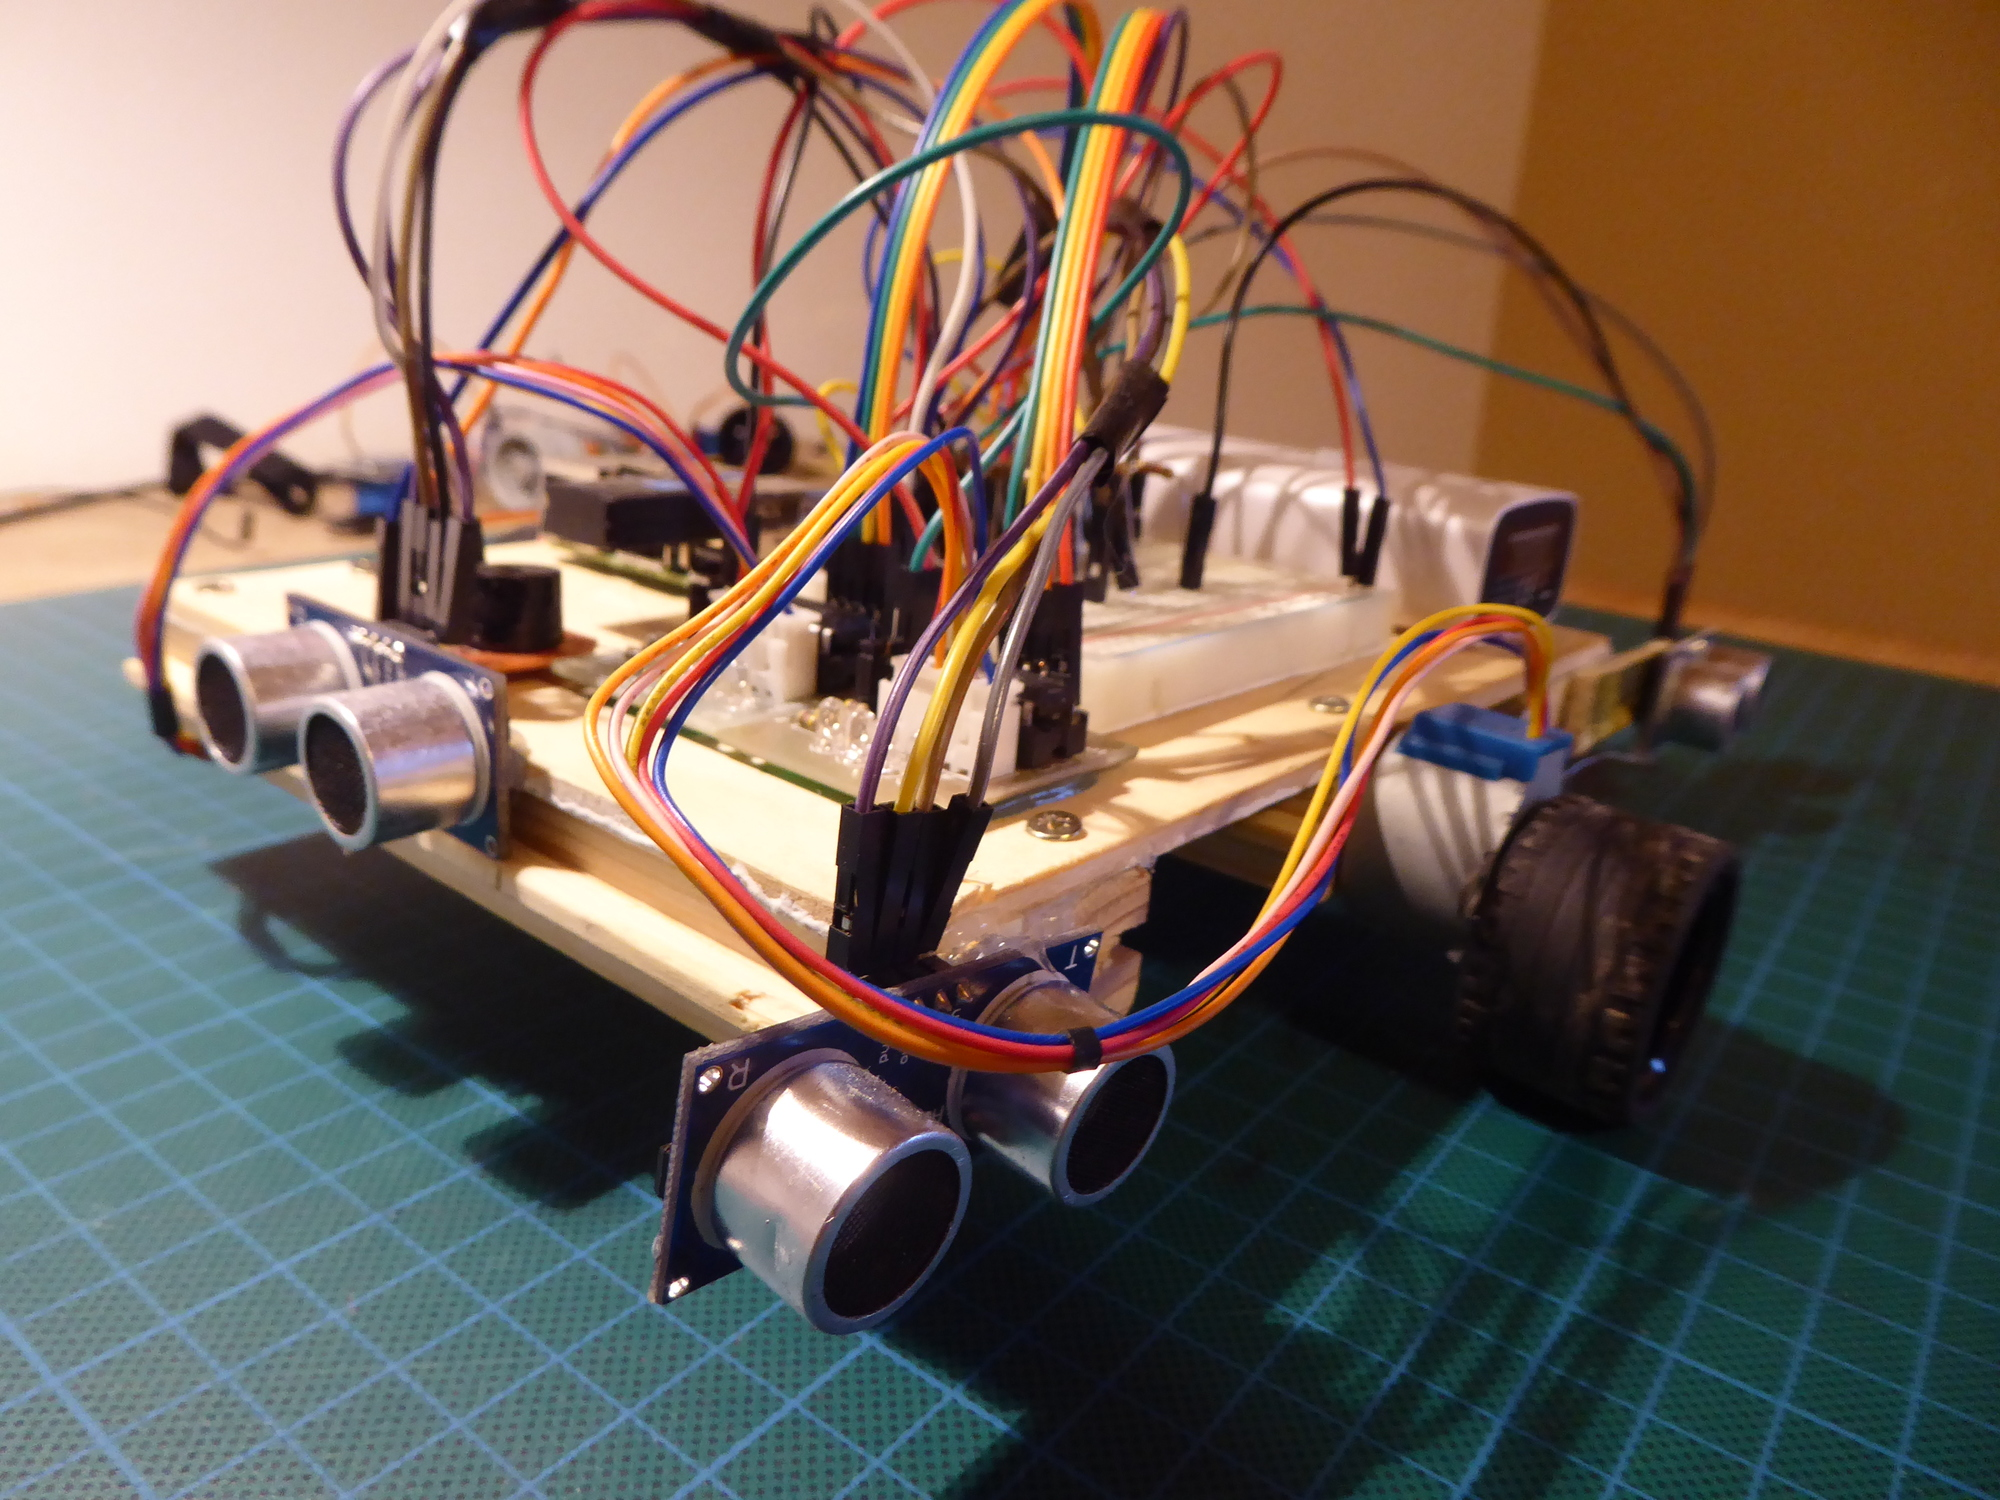
\includegraphics[width=15cm]{robo}\\[0.5cm]
\hallo{Eine neue Ära der Messkunst (ziemlich scheisse!)}
\end{center}
\thispagestyle{empty}
\newpage

\tableofcontents
\newpage

\section{Vorgehensweise}
\vspace{0.3cm}
\renewcommand{\baselinestretch}{1.3}%

\begin{wrapfigure}{r}{8cm}%
	\xbox(*,-5.5ex)[b]{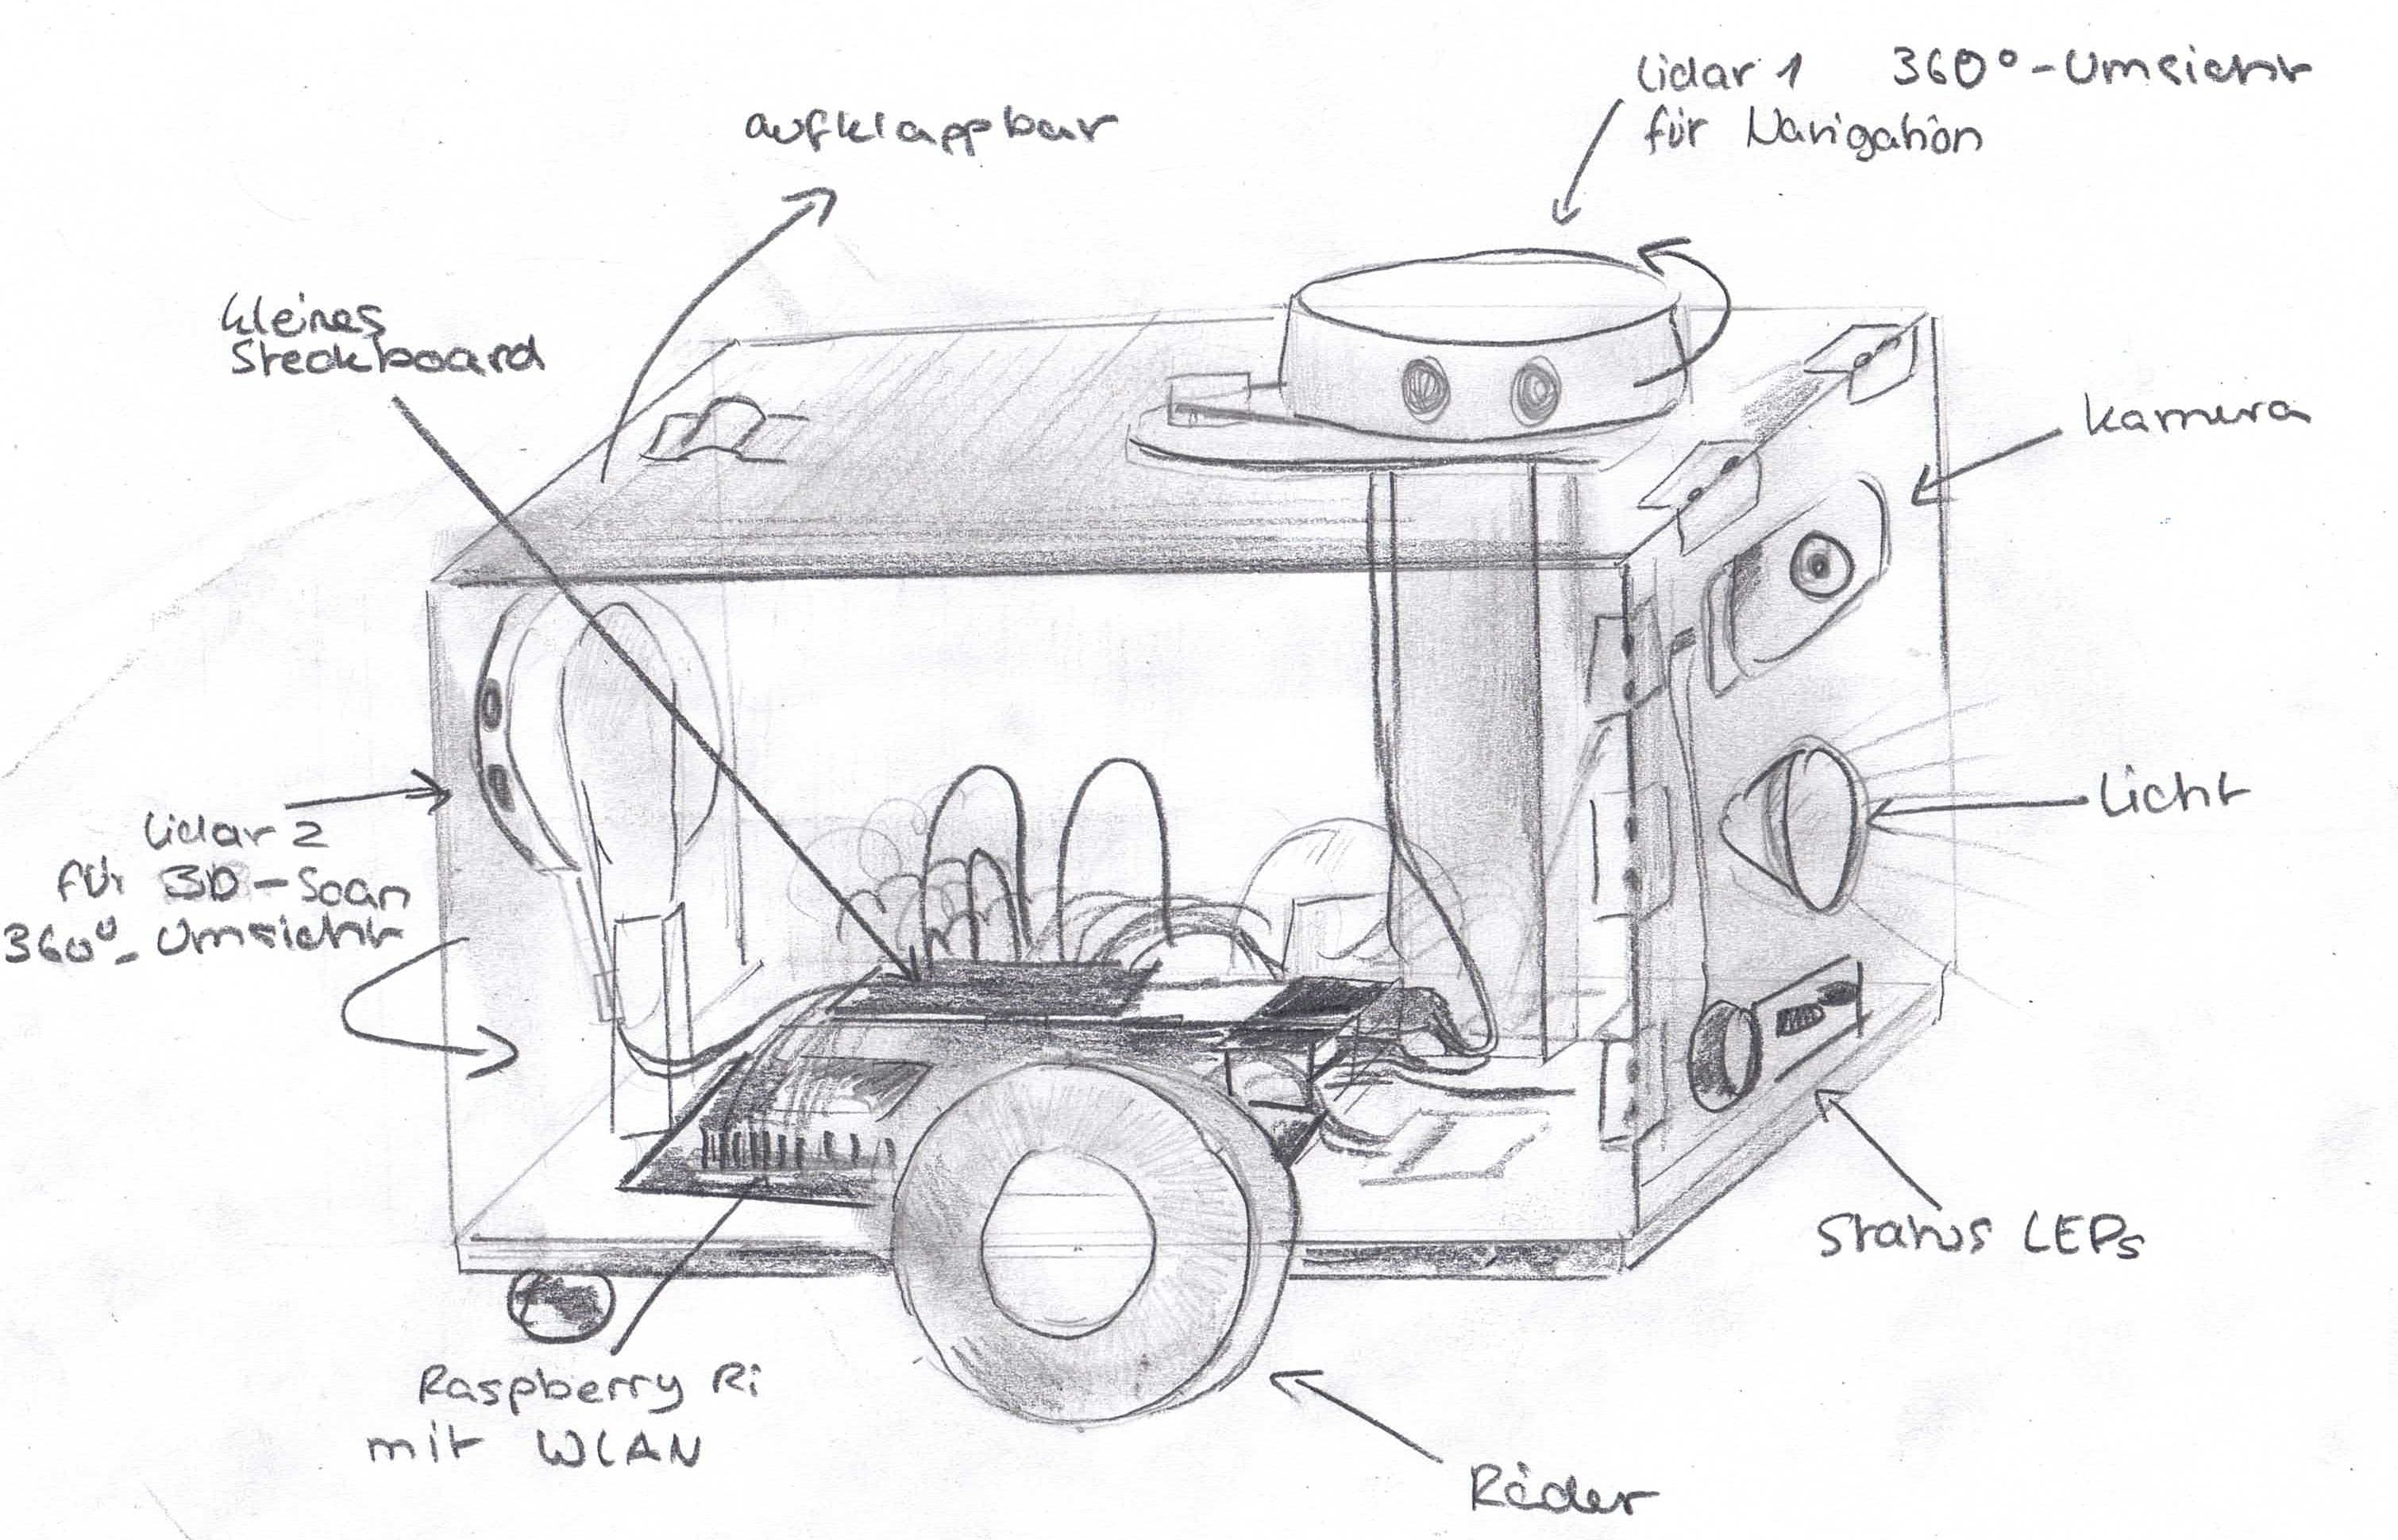
\includegraphics[width=\linewidth]{bild1}}%
	\caption{\sf Unser erster Entwurf}%
\end{wrapfigure}

\textsf{%
	Da wir letztes Jahr schon mit diesem Projekt angetreten sind, ist das Projekt eine Weiterführung.
	\\[3mm]
	Wie verteilten die Aufgaben folgenderma\ss en: Kolja kümmert sich um das Schassi und die Verkabelung und Maxi um die Programmierung (GUI, Raspberry Pi).\\[3mm]
	Zuerst überlegten wir uns, wie der Roboter eingentlich aussehen sollte und was wichtig wäre. Unser erster Entwurf sah folgendermaßen aus:
}

\section{Mathematik}
\subsection{3D-Darstellung}
\vspace{0.8cm}
\begin{center}
	\begin{tabular}{c}
		\xbox[t]{%
			\begin{tikzpicture}[
				mylabel/.style 2 args={scale=#2, rounded corners=0.7mm,
					fill=#1, draw=black,
					ultra thin, inner sep=0.7mm},
				o/.style 2 args={fill=#1, fill opacity=#2},
				scale=1.0
				]
				\begin{scope}[tdplot_main_coords]
					\tdplotsetrotatedcoords{-120}{35}{126}
					%
					\begin{scope}[tdplot_rotated_coords, every node/.style={font=\tiny}, node distance=0.15mm]
						\pgfmathsetmacro{\s}{1.5}
						\pgfmathsetmacro{\a}{3.2}
						%
						\coordinate (origin) at (0,0,0);
						\coordinate (p1) at (\s,\s,\s);
						\coordinate (p2) at (\s,-\s,\s);
						\coordinate (p3) at (-\s,-\s,\s);
						\coordinate (p4) at (-\s,\s,\s);
						%
						\coordinate (p5) at (\s,\s,-\s);
						\coordinate (p6) at (\s,-\s,-\s);
						\coordinate (p7) at (-\s,-\s,-\s);
						\coordinate (p8) at (-\s,\s,-\s);
						%
						\coordinate(xaxis) at (\a,0,0);
						\coordinate(yaxis) at (0,\a,0);
						\coordinate(zaxis) at (0,0,1.8*\a);
						%
						\begin{scope}[thick]
							\draw (p1) -- (p2) -- (p3) -- (p4) -- cycle;
							\draw (p5) -- (p6) -- (p7) -- (p8) -- cycle;
							\draw (p1) -- (p5) (p2) -- (p6) (p3) -- (p7) (p4) -- (p8);
							%
							\fill[o={black}{0.2}] (p1) -- (p2) -- (p3) -- (p4) -- cycle;
							\fill[o={black}{0.35}] (p1) -- (p4) -- (p8) -- (p5) -- cycle;
							\fill[o={black}{0.5}] (p1) -- (p5) -- (p6) -- (p2) -- cycle;
						\end{scope}
						%
						\begin{scope}[thick, draw=purple, node distance=0pt, text=purple, every node/.style={scale=1}]
							\draw[->] (origin) -- (zaxis);
							\draw[->] (origin) -- (xaxis);
							\draw[->] (origin) -- (yaxis);
							%
							\node[right=of xaxis] {$x$};
							\node[above=of yaxis] {$y$};
							\node[below left=of zaxis] {$z$};
						\end{scope}
						%
						\begin{scope}[every node/.style={fill opacity=0.85, text opacity=1}]
							\foreach \i/\tt in {1/1|1|1, 2/1|-1|1, 3/-1|-1|1, 4/-1|1|1, 5/1|1|-1, 6/1|-1|-1, 7/-1|-1|-1, 8/-1|1|-1} {
								\node (n\i) at (p\i) [shape=circle, inner sep=0.5mm, text=white, fill=black, text=white, scale=0.8] {\i};
								\node (s\i) [mylabel={white}{0.67}, rounded corners=1.8mm, inner sep=1.3mm, below=of n\i] {\tt};
							}
						\end{scope}
						%
						\node(norigin) at (origin) [circle, fill=red, text width=1mm, inner sep=0pt, draw=black, fill=yellow] {};
						\node(noriginl) [mylabel={yellow!50!white}{1}, rounded corners=1.3mm, inner sep=1mm, fill opacity=0.7, text opacity=1, below=of norigin, scale=0.95] {0|0|0};
					\end{scope}
				\end{scope}
				%
				\begin{scope}[xshift=-6cm]
					\tdplotsetrotatedcoords{-120}{40}{126}
					%
					\begin{scope}[tdplot_rotated_coords, every node/.style={font=\tiny}, node distance=0.15mm]
						\pgfmathsetmacro{\s}{1.5}
						\pgfmathsetmacro{\a}{3.2}
						%
						\coordinate (origin) at (0,0,0);
						\coordinate (p1) at (\s,\s,\s);
						\coordinate (p2) at (\s,-\s,\s);
						\coordinate (p3) at (-\s,-\s,\s);
						\coordinate (p4) at (-\s,\s,\s);
						%
						\coordinate (p5) at (\s,\s,-\s);
						\coordinate (p6) at (\s,-\s,-\s);
						\coordinate (p7) at (-\s,-\s,-\s);
						\coordinate (p8) at (-\s,\s,-\s);
						%
						\coordinate(xaxis) at (\a,0,0);
						\coordinate(yaxis) at (0,\a,0);
						\coordinate(zaxis) at (0,0,1.6*\a);
						%
						\begin{scope}[on background layer]
							\fill[o={black!20!green}{0.4}] (p1) -- (p2) -- (p3) -- (p4) -- cycle;
							\fill[o={black!35!red}{0.5}] (p1) -- (p4) -- (p8) -- (p5) -- cycle;
							\fill[o={black!60!blue}{0.6}] (p1) -- (p5) -- (p6) -- (p2) -- cycle;
						\end{scope}
						%
						\begin{scope}[thick, draw=purple, node distance=0pt, text=purple, every node/.style={scale=1}]
							\draw[->] (origin) -- (zaxis);
							\draw[->] (origin) -- (xaxis);
							\draw[->] (origin) -- (yaxis);
							%
							\node[right=of xaxis] {$x$};
							\node[above=of yaxis] {$y$};
							\node[below left=of zaxis] {$z$};
						\end{scope}
						%
						\begin{scope}[every node/.style={fill opacity=0.85, text opacity=1}]
							\foreach \i in {1,...,8}
							\node (n\i) at (p\i) [shape=circle, inner sep=0.5mm, text=white, fill=black, text=white, scale=0.8] {\i};
						\end{scope}
						%
						\begin{scope}[every node/.style={inner sep=1.5mm, rounded corners=2mm, text=white, scale=0.8}]
							\node at (1.5,0,0) [fill=blue] {\sf\small 1-5-6-2-1};
							\node at (0.3,0,2) [fill=black!40!green] {\sf\small 1-2-3-4-1};
							\node at (0,1.5,0) [fill=black!20!red] {\sf\small 5-1-4-8-5};
						\end{scope}
						%
						\node(norigin) at (origin) [circle, fill=red, text width=1mm, inner sep=0pt, draw=black, fill=yellow] {};
						%
						\begin{scope}[on background layer]
							\begin{scope}[thick, >={Stealth[round, length=3.5mm]}]
								\draw[->] (n1) -- (n2); \draw[->] (n2) -- (n3); \draw[->] (n3) -- (n4); \draw[->] (n4) -- (n1);
								\draw (n5) -- (n6); \draw (n6) -- (n7); \draw (n7) -- (n8); \draw (n8) -- (n5);
								\draw (n5) -- (n1); \draw (n6) -- (n2); \draw (n3) -- (n7); \draw (n4) -- (n8);
							\end{scope}
						\end{scope}
					\end{scope}
				\end{scope}
			\end{tikzpicture}%
		}
		\\
		\xbox[t](+1cm,+1cm){%
			\begin{tikzpicture}
				\node(text) [node distance=0mm, right=of xaxis, inner sep=3mm, rounded corners=3mm, fill=black!12!white, text width=9cm] {
					\renewcommand{\baselinestretch}{1.0}%
					\begin{minipage}{9cm}
						\sf\small Jedes Objekt wird durch Eckpunkte und Flächen beschrieben.\\[2mm]
						Die Position eines jeden Objektes beträgt anfangs $(0|0|0)$. Die Eckpunkte werden relativ zur Position des Objektes angegeben. Alle Punkte werden nun mit einer Ziffer versehen, damit man die Flächen beschreiben kann.
					\end{minipage}
				};
			\end{tikzpicture}%
		}
	\end{tabular}
\begin{wraptable}{8cm}
	\begin{minipage}{8cm}
		\begin{tikzpicture}[
			tdplot_main_coords,
			mylabel/.style 2 args={scale=#2, rounded corners=0.7mm,
			fill=#1, draw=black,
			ultra thin, inner sep=0.7mm},
			o/.style 2 args={fill=#1, fill opacity=#2},
			]
			\tdplotsetrotatedcoords{-120}{35}{126}
			%
			\begin{scope}[tdplot_rotated_coords, every node/.style={font=\tiny}, node distance=0.15mm]
				\pgfmathsetmacro{\s}{1.5}
				\pgfmathsetmacro{\a}{3.2}
				%
				\coordinate (origin) at (0,0,0);
				\coordinate (p1) at (\s,\s,\s);
				\coordinate (p2) at (\s,-\s,\s);
				\coordinate (p3) at (-\s,-\s,\s);
				\coordinate (p4) at (-\s,\s,\s);
				%
				\coordinate (p5) at (\s,\s,-\s);
				\coordinate (p6) at (\s,-\s,-\s);
				\coordinate (p7) at (-\s,-\s,-\s);
				\coordinate (p8) at (-\s,\s,-\s);
				%
				\coordinate(xaxis) at (\a,0,0);
				\coordinate(yaxis) at (0,\a,0);
				\coordinate(zaxis) at (0,0,1.6*\a);
				%
				\begin{scope}[thick]
					\draw (p1) -- (p2) -- (p3) -- (p4) -- cycle;
					\draw (p5) -- (p6) -- (p7) -- (p8) -- cycle;
					\draw (p1) -- (p5) (p2) -- (p6) (p3) -- (p7) (p4) -- (p8);
				\end{scope}
				%
				\fill[o={black!20!green}{0.4}] (p1) -- (p2) -- (p3) -- (p4) -- cycle;
				\fill[o={black!35!red}{0.5}] (p1) -- (p4) -- (p8) -- (p5) -- cycle;
				\fill[o={black!60!blue}{0.6}] (p1) -- (p5) -- (p6) -- (p2) -- cycle;
				%
				\begin{scope}[thick, draw=purple, node distance=0pt, text=purple, every node/.style={scale=1}]
					\draw[->] (origin) -- (zaxis);
					\draw[->] (origin) -- (xaxis);
					\draw[->] (origin) -- (yaxis);
					%
					\node[right=of xaxis] {$x$};
					\node[above=of yaxis] {$y$};
					\node[below left=of zaxis] {$z$};
				\end{scope}
				%
				\begin{scope}[very thick, >={Stealth[round, length=3.5mm]}, node distance=-1mm]
					\node(c) at (0,0,1.5) [shape=circle, inner sep=0pt, text width=6mm] {};
					\draw[->] (-1.5,0,-1.5) .. controls (-3.5,0,-1.5) and (-3.5,0,1.5) .. node(zy) {} (c);
					\draw[->] (0,0,-1.5) .. controls (0,3.5,-1.5) and (0,3.5,1.5) .. node(zx) {} (c);
					\node[left=of zy] {\small $y:5^\circ$};
					\node[above right=of zx] {\small $x:20^\circ$};
					\filldraw[thin, draw=black, fill=orange] (p1) circle[radius=1mm];
				\end{scope}
				%
				\node(norigin) at (origin) [circle, fill=red, text width=1mm, inner sep=0pt, draw=black, fill=yellow] {};
				%
				\tdplotsetrotatedcoords{-102}{51}{109}
				%
				\begin{scope}[yshift=-5cm, tdplot_rotated_coords]
					\draw[->, thick, dashed] (p2) ++(0.35cm,0.5mm) .. controls (40:2.7cm) .. node(nnn){} (1.5cm,4mm);
					%
					\pgfmathsetmacro{\s}{1}
					\pgfmathsetmacro{\a}{2.5}
					%
					\coordinate (origin) at (0,0,0);
					\coordinate (p1) at (\s,\s,\s);
					\coordinate (p2) at (\s,-\s,\s);
					\coordinate (p3) at (-\s,-\s,\s);
					\coordinate (p4) at (-\s,\s,\s);
					%
					\coordinate (p5) at (\s,\s,-\s);
					\coordinate (p6) at (\s,-\s,-\s);
					\coordinate (p7) at (-\s,-\s,-\s);
					\coordinate (p8) at (-\s,\s,-\s);
					%
					\coordinate(xaxis) at (\a,0,0);
					\coordinate(yaxis) at (0,1.2*\a,0);
					\coordinate(zaxis) at (0,0,\a);
					%
					\begin{scope}[thick]
						\draw (p1) -- (p2) -- (p3) -- (p4) -- cycle;
						\draw (p5) -- (p6) -- (p7) -- (p8) -- cycle;
						\draw (p1) -- (p5) (p2) -- (p6) (p3) -- (p7) (p4) -- (p8);
					\end{scope}
					%
					\fill[o={black!20!green}{0.4}] (p1) -- (p2) -- (p3) -- (p4) -- cycle;
					\fill[o={black!35!red}{0.5}] (p1) -- (p4) -- (p8) -- (p5) -- cycle;
					\fill[o={black!60!blue}{0.6}] (p1) -- (p5) -- (p6) -- (p2) -- cycle;
					%
					\begin{scope}[thick, draw=purple, node distance=0pt, text=purple, every node/.style={scale=1}]
						\draw[->] (origin) -- (zaxis);
						\draw[->] (origin) -- (xaxis);
						\draw[->] (origin) -- (yaxis);
						%
						\node[right=of xaxis] {$x$};
						\node[above=of yaxis] {$y$};
						\node[below left=of zaxis] {$z$};
					\end{scope}
				\end{scope}
			\end{scope}
		\end{tikzpicture}
	\end{minipage}
	\caption{\sf Unser erster Entwurf}%
\end{wraptable}
\begin{raggedright}
	{
		\sf\small Um das Objekt nun zu drehen, muss man alle Punkte des Objektes mit den folgenden Drehmatritzen multiplizieren:\\[5mm]
		%
		\begin{tabular}{lr}
			\textbf{\footnotesize X-Drehung:}&
			$
			\left(\begin{array}{ccc}
				1 & 0 & 0 \\
				0 & \cos\alpha & -\sin\alpha\\
				0 & \sin\alpha & \cos\alpha
			\end{array}\right)
			$\\[6mm]
			\textbf{\footnotesize Y-Drehung:}&
			$
			\left(\begin{array}{ccc}
				\cos\alpha & 0 & \sin\alpha \\
				0 & 1 & 0 \\
				-\sin\alpha & 0 & \cos\alpha
			\end{array}\right)
			$\\[6mm]
			\textbf{\footnotesize Z-Drehung:}&
			$
			\left(\begin{array}{ccc}
				\cos\alpha & -\sin\alpha & 0 \\
				\sin\alpha & \cos\alpha & 0 \\
				0 & 0 & 1 \\
			\end{array}\right)
			$\\[6mm]
		\end{tabular}\\[5mm]
		\textbf{Beispiel:}\\[2mm]
		Um nun den Punkt $(1|1|1)$ (links orange) $20^\circ$ um die X-Achse und $5^\circ$ um die Y-Achse zu drehen muss man folgendes rechnen:\\[2mm]
		\[
		\left(\begin{array}{ccc}
			\cos 5^\circ & 0 & \sin 5^\circ \\
			0 & 1 & 0 \\
			-\sin 5^\circ & 0 & \cos 5^\circ
		\end{array}\right)
		\cdot
		\left(\begin{array}{ccc}
			1 & 0 & 0 \\
			0 & \cos 20^\circ & -\sin 20^\circ\\
			0 & \sin 20^\circ & \cos 20^\circ
		\end{array}\right)
		\cdot
		\left(\begin{array}{ccc}
			1\\1\\1
		\end{array}\right)
		\]
	}
\end{raggedright}

\begin{minipage}{10cm}
	\begin{tikzpicture}
		\tdplotsetrotatedcoords{-67}{43}{60}
		\begin{scope}[tdplot_rotated_coords]
			%
			\pgfmathsetmacro{\s}{2}
			\pgfmathsetmacro{\a}{4}
			%
			\coordinate (p1) at (\s,0,-\s);
			\coordinate (p2) at (\s,0,\s);
			\coordinate (p3) at (-\s,0,\s);
			\coordinate (p4) at (-\s,0,-\s);
			\coordinate (origin) at (0,0,0);
			%
			\coordinate(xaxis) at (\a,0,0);
			\coordinate(yaxis) at (0,1.25*\a,0);
			\coordinate(zaxis) at (0,0,\a);
			\coordinate(oxaxis) at (-\a,0,0);
			\coordinate(oyaxis) at (0,-\a,0);
			\coordinate(ozaxis) at (0,0,-\a);
			\coordinate(t) at (0,3.5,0);
			%
			\begin{scope}
				\filldraw[thick, fill=black!20!yellow, draw=black] (p1) -- (p2) -- (p3) -- (p4) -- (p1);
				%
				\begin{scope}[thick, draw=purple, node distance=0pt, text=purple, every node/.style={scale=1}]
					\draw[->] (ozaxis) -- (zaxis);
					\draw[->] (oxaxis) -- (xaxis);
					\draw[->] (oyaxis) -- (yaxis);
					%
					\node[right=of xaxis] {$x$};
					\node[above=of yaxis] {$y$};
					\node[below left=of zaxis] {$z$};
				\end{scope}
				%
				\begin{scope}[
					every node/.style={thin, shape=circle,inner sep=0pt,text width=2mm, fill=red, draw=black},
					]
					\node at (p1) [label={[label distance=1mm]above:{$A$}}] {};
					\node at (p2) [label={[label distance=1mm]below:{$B$}}] {};
					\node at (p3) [label={[label distance=1mm]below:{$C$}}] {};
					\node at (p4) [label={[label distance=1mm]above:{$D$}}] {};
				\end{scope}
				%
				\node(L) at (3.5,3,-1) [shape=circle, inner sep=1mm, fill=yellow, draw=black, thin, label=right:{\sf\footnotesize Licht}] {$L$};
				%
				\begin{scope}[very thick, >={Stealth[round, length=3.5mm]}]
					\coordinate(uu) at (-1.5,0,0);
					%
					\pic["$\alpha$", draw=black, fill=green, angle eccentricity=0.7, angle radius=1cm] {angle=L--origin--t};
					\pic[thin,"$\cdot$", draw=black, fill=yellow, angle eccentricity=0.4, angle radius=0.4cm] {angle=t--origin--uu};
					\draw[thin] (origin) -- (uu);
					%
					\draw[->] (origin) -- node[near end, label={[label distance=1mm]left:{\large $\vec{u}$}}, align=left] {} (L);
					\draw[->](origin) -- node[near end, label={[label distance=-1mm]left:{\large $\vec{v}$}}, align=left] {} (t);
				\end{scope}
			\end{scope}
		\end{scope}
	\end{tikzpicture}
\end{minipage}
\\[1cm]
\begin{raggedright}
	\sf\small Um nun auch noch Lichter mit beliebiger Farbe im Raum platzieren zu können, muss man die Farben der Flächen zu allen Lichtern berechnen. Dazu braucht man den Normalenvektor $\vec{v}$. Diesen erhält man durch das Vektorprodukt:
	\\[-2mm]
	\[
	\vec{a}=A-B\hspace{5mm}\vec{b}=B-C
	\]
	\[
	\vec{v} = \vec{a}\times \vec{b} =
	\left(\begin{array}{ccc}a_1\\a_2\\a_3\end{array}\right)\times
	\left(\begin{array}{ccc}b_1\\b_2\\b_3\end{array}\right)=
	\left(\begin{array}{ccc}
		a_2 b_2 - a_3 b_2\\
		a_3 b_1 - a_1 b_3\\
		a_1 b_2 - a_2 b_1\\
	\end{array}\right)
	\]\\[5mm]
	Durch das Vektorprodukt haben wir nun den Normalenvektor $\vec{v}$ der Fläche $ABCD$ berechnet. Nun kann man die Gewichtung $f$ des Lichtes auf die Fläche wie folgt berechnen:
	\\[-3mm]
	\begin{eqnarray*}
		\vec{u}\cdot\vec{v} = \left(
		\begin{array}{ccc}u_1\\u_2\\u_3\end{array} \right) \cdot \left(
		\begin{array}{ccc}v_1\\v_2\\v_3\end{array}
		\right) = u_1 \cdot v_1 + u_2 \cdot v_2 + u_3 \cdot v_3\\[2mm]
		\alpha = \cos^{-1}\left(\frac{\displaystyle |\vec{u}\cdot\vec{v}|}{\displaystyle |\vec{u}|\cdot|\vec{v}|}\right)
		\hspace{2mm}\Rightarrow\hspace{2mm}
		f = \cos\alpha = \frac{\displaystyle |\vec{u}\cdot\vec{v}|}{\displaystyle |\vec{u}|\cdot|\vec{v}|}
	\end{eqnarray*}
	\\[3mm]
	Zuletzt muss man folgendes auf alle Lichter anwenden:\\[2mm]
	%
	\begin{center}
		\begin{tabular}{r|l}
			$r,g,b$ & aktuelle Farbe der Fläche (Anfang: $1,1,1$)\\
			$f$ & oben berechneter Faktor\\
			$L_r,L_g,L_b$ & Farben der Lichter
		\end{tabular}
	\end{center}
	\vspace{-5mm}
	%
	\[
	r,g,b,L_r,L_g,L_b \in[0;1]
	\]
	\[
	r=1-(1-r)\cdot(1-f\cdot L_r)
	\]
	\[
	g=1-(1-g)\cdot(1-f\cdot L_g)
	\]
	\[
	b=1-(1-b)\cdot(1-f\cdot L_b)
	\]
\end{raggedright}
\begin{tabular}{rl}
	\xbox[t](*,+2cm) {
		\begin{tikzpicture}[scale=0.9]
			\tdplotsetrotatedcoords{-120}{35}{126}
			\begin{scope}[
				tdplot_rotated_coords,
				o/.style 2 args={fill=#1, fill opacity=#2}
				]
				%
				\pgfmathsetmacro{\s}{0.6}
				\pgfmathsetmacro{\ss}{0.8}
				\pgfmathsetmacro{\a}{3}
				%
				\pgfmathsetmacro{\x}{3}
				\pgfmathsetmacro{\y}{2}
				\pgfmathsetmacro{\z}{-2}
				%
				\coordinate (qorigin) at (\x,\y,\z);
				\coordinate (p1) at (\x+\s,\y+\s,\z+\s);
				\coordinate (p2) at (\x+\s,\y-\s,\z+\s);
				\coordinate (p3) at (\x-\s,\y-\s,\z+\s);
				\coordinate (p4) at (\x-\s,\y+\s,\z+\s);
				%
				\coordinate (p5) at (\x+\s,\y+\s,\z-\s);
				\coordinate (p6) at (\x+\s,\y-\s,\z-\s);
				\coordinate (p7) at (\x-\s,\y-\s,\z-\s);
				\coordinate (p8) at (\x-\s,\y+\s,\z-\s);
				%
				\coordinate (origin) at (0,0,0);
				%
				\coordinate (pp1) at (\ss,\ss,\ss);
				\coordinate (pp2) at (\ss,-\ss,\ss);
				\coordinate (pp3) at (-\ss,-\ss,\ss);
				\coordinate (pp4) at (-\ss,\ss,\ss);
				%
				\coordinate (pp5) at (\ss,\ss,-\ss);
				\coordinate (pp6) at (\ss,-\ss,-\ss);
				\coordinate (pp7) at (-\ss,-\ss,-\ss);
				\coordinate (pp8) at (-\ss,\ss,-\ss);
				%
				\coordinate(xaxis) at (\a,0,0);
				\coordinate(yaxis) at (0,1.25*\a,0);
				\coordinate(zaxis) at (0,0,\a);
				\coordinate(oxaxis) at (-\a,0,0);
				\coordinate(oyaxis) at (0,-\a,0);
				\coordinate(ozaxis) at (0,0,-\a);
				%
				\coordinate(t) at (0,3.5,0);
				%
				\begin{scope}[thick]
					\draw (p1) -- (p2) -- (p3) -- (p4) -- cycle;
					\draw (p5) -- (p6) -- (p7) -- (p8) -- cycle;
					\draw (p1) -- (p5) (p2) -- (p6) (p3) -- (p7) (p4) -- (p8);
				\end{scope}
				%
				\fill [o={black!20!green}{0.4}] (p1) -- (p2) -- (p3) -- (p4) -- cycle;
				\fill [o={black!35!red}{0.5}] (p1) -- (p4) -- (p8) -- (p5) -- cycle;
				\fill [o={black!60!blue}{0.6}] (p1) -- (p5) -- (p6) -- (p2) -- cycle;
				%
				\begin{scope}[thin]
					\draw[dashed] (pp1) -- (pp2) -- (pp3) -- (pp4) -- cycle;
					\draw[dashed] (pp5) -- (pp6) -- (pp7) -- (pp8) -- cycle;
					\draw[dashed] (pp1) -- (pp5) (pp2) -- (pp6) (pp3) -- (pp7) (pp4) -- (pp8);
				\end{scope}
				%
				\fill [o={black!20!green}{0.2}] (pp1) -- (pp2) -- (pp3) -- (pp4) -- cycle;
				\fill [o={black!35!red}{0.3}] (pp1) -- (pp4) -- (pp8) -- (pp5) -- cycle;
				\fill [o={black!60!blue}{0.4}] (pp1) -- (pp5) -- (pp6) -- (pp2) -- cycle;
				%
				\begin{scope}[thick, draw=purple, node distance=0pt, text=purple, every node/.style={scale=1}]
					\draw[->] (ozaxis) -- (zaxis);
					\draw[->] (oxaxis) -- (xaxis);
					\draw[->] (oyaxis) -- (yaxis);
					%
					\node[right=of xaxis] {$x$};
					\node[above=of yaxis] {$y$};
					\node[below left=of zaxis] {$z$};
				\end{scope}
				%
				\begin{scope}[every node/.style={shape=circle, inner sep=0pt, fill=orange, draw=black, thin}]
					\node (nqorigin) at (qorigin) [text width=1.5mm] {};
					\node (norigin) at (origin) [text width=2mm] {};
				\end{scope}
				\draw [thick, ->, draw=black!50!blue] (norigin) -- node [label={[label 	distance=0mm]right:{$\vec{v}$}}] {} (nqorigin);
				%
				\node at (p4) [shape=circle, inner sep=0, text width=1mm, label={left:{$Q'$}}] {};
				%
				\node at (pp4) [shape=circle, inner sep=0, text width=1mm, label={left:{$Q$}}] {};
			\end{scope}
		\end{tikzpicture}
	}
	&
	\xbox[t](+2cm,+1cm) {
		\begin{tikzpicture}
			\node(text) [node distance=15mm, right=of xaxis, inner sep=5mm, rounded corners=3mm, fill=black!12!white, text width=9cm] {
				\begin{minipage}{9cm}
					\renewcommand{\baselinestretch}{1.0}%
					\sf\small
					Um nun eine Translation (Verschiebung) vorzunehmen muss man den Vektor $\vec{v}$ zu allen Punkten des Objektes $Q$ addieren. Jetzt will man natürlich eine Transformation auch mit einer Matrix beschreiben können. Um dies vorzunehemen muss man die Matrix um eine Zeile und eine Spalte erweitern. Alle Vektoren müssen dann auch um eine Koordinate mit dem Wert $1$ erweitert werden:
					\begin{eqnarray*}
						\vec{p} & = & \textrm{\sf Ortsvektor zu jedem Punkt des Objektes $Q$}\\
						\vec{p'}& = & \textrm{\sf Ortsvektor zu jedem Punkt des Objektes $Q'$}
					\end{eqnarray*}
					\[
					\vec{p'} = \vec{p} + \vec{v} =
					\left(
					\begin{array}{cccc}
						1 & 0 & 0 & v_1 \\
						0 & 1 & 0 & v_2 \\
						0 & 0 & 1 & v_3 \\
						0 & 0 & 0 & 1
					\end{array}
					\right)\cdot
					\left(
					\begin{array}{c}p_1\\p_2\\p_3\\1\end{array}
					\right)
					\]
					\xbox{\textbf{Beispiel:}}(0,-5pt)\\
					Um den Punkt $(0|3|2)$ um den Vektor $\left(\begin{array}{c}3\\1\\2\end{array}\right)$ zu verschieben:\\
					\begin{eqnarray*}
						p'& = &
						\left(
						\begin{array}{cccc}
							1 & 0 & 0 & 3 \\
							0 & 1 & 0 & 1 \\
							0 & 0 & 1 & 2 \\
							0 & 0 & 0 & 1
						\end{array}
						\right)\cdot
						\left(
						\begin{array}{c}0\\3\\2\\1\end{array}
						\right)\\[1mm]
						& = &
						\left(
						\begin{array}{c}
							1\cdot 0 + 0\cdot 3 + 0\cdot 2 + 3\cdot 1 \\
							0\cdot 0 + 1\cdot 3 + 0\cdot 2 + 1\cdot 1 \\
							0\cdot 0 + 0\cdot 3 + 1\cdot 2 + 2\cdot 1 \\
							0\cdot 0 + 0\cdot 3 + 0\cdot 2 + 1\cdot 1
						\end{array}
						\right)
						=
						\left(
						\begin{array}{c}
							3\\4\\4\\1
						\end{array}
						\right)
					\end{eqnarray*}
				\end{minipage}
			};
		\end{tikzpicture}
	}
\end{tabular}
\begin{longtable}{c}
\\[0.5cm]
		\begin{tikzpicture}[
			o/.style 2 args={fill=#1, fill opacity=#2}
			]
			%
			\tdplotsetrotatedcoords{-120}{35}{126}
			\begin{scope}[tdplot_rotated_coords]
				\pgfmathsetmacro{\ss}{0.8}
				\pgfmathsetmacro{\a}{3}
				%
				\coordinate (origin) at (0,0,0);
				%
				\coordinate (p1) at (\ss,\ss,\ss);
				\coordinate (p2) at (\ss,-\ss,\ss);
				\coordinate (p3) at (-\ss,-\ss,\ss);
				\coordinate (p4) at (-\ss,\ss,\ss);
				%
				\coordinate (p5) at (\ss,\ss,-\ss);
				\coordinate (p6) at (\ss,-\ss,-\ss);
				\coordinate (p7) at (-\ss,-\ss,-\ss);
				\coordinate (p8) at (-\ss,\ss,-\ss);
				%
				\coordinate(xaxis) at (\a,0,0);
				\coordinate(yaxis) at (0,1.25*\a,0);
				\coordinate(zaxis) at (0,0,\a);
				\coordinate(oxaxis) at (-\a,0,0);
				\coordinate(oyaxis) at (0,-\a,0);
				\coordinate(ozaxis) at (0,0,-\a);
				%
				\fill [o={black!20!green}{0.4}] (p1) -- (p2) -- (p3) -- (p4) -- cycle;
				\fill [o={black!35!red}{0.5}] (p1) -- (p4) -- (p8) -- (p5) -- cycle;
				\fill [o={black!60!blue}{0.6}] (p1) -- (p5) -- (p6) -- (p2) -- cycle;
				%
				\begin{scope}[thick, draw=purple, node distance=0pt, text=purple, every node/.style={scale=1}]
					\draw[->] (ozaxis) -- (zaxis);
					\draw[->] (oxaxis) -- (xaxis);
					\draw[->] (oyaxis) -- (yaxis);
					%
					\node[right=of xaxis] {$x$};
					\node[above=of yaxis] {$y$};
					\node[below left=of zaxis] {$z$};
				\end{scope}
				%
				\begin{scope}[thin]
					\draw (p1) -- (p2) -- (p3) -- (p4) -- cycle;
					\draw (p5) -- (p6) -- (p7) -- (p8) -- cycle;
					\draw (p1) -- (p5) (p2) -- node[circle, inner sep=0pt, text width=1.5mm, label=right:{$Q$}] {} (p6) (p3) -- (p7) (p4) -- (p8);
				\end{scope}
				%
				\begin{scope}[every node/.style={shape=circle, inner sep=0pt, fill=orange, draw=black, thin}]
					\node (norigin) at (origin) [text width=1.5mm] {};
				\end{scope}
			\end{scope}
			%
			\tdplotsetrotatedcoords{-148}{70}{160}
			\begin{scope}[tdplot_rotated_coords]
				\pgfmathsetmacro{\ga}{0.2}
				\pgfmathsetmacro{\gb}{0.5}
				%
				\pgfmathsetmacro{\cd}{4.5}
				\pgfmathsetmacro{\cs}{1.2}
				%
				\coordinate (k1) at (\ga,\ga,\cd);
				\coordinate (k2) at (\ga,-\ga,\cd);
				\coordinate (k3) at (-\ga,-\ga,\cd);
				\coordinate (k4) at (-\ga,\ga,\cd);
				%
				\coordinate (k5) at (\gb,\gb,\cd-\cs);
				\coordinate (k6) at (\gb,-\gb,\cd-\cs);
				\coordinate (k7) at (-\gb,-\gb,\cd-\cs);
				\coordinate (k8) at (-\gb,\gb,\cd-\cs);
				%
				\coordinate (ko) at (0,0,\cd-\cs/2);
				%
				\begin{scope}[thin]
					\draw (k1) -- (k2) -- (k3) -- (k4) -- cycle;
					\draw (k5) -- (k6) -- (k7) -- (k8) -- cycle;
					\draw (k1) -- (k5) (k2) -- node[circle, inner sep=0pt, text width=1.5mm, label=below:{$K$}] {} (k6) (k3) -- (k7) (k4) -- (k8);
					%
					\fill [fill=black, fill opacity=0.25] (k1) -- (k2) -- (k6) -- (k5);
					\fill [fill=black, fill opacity=0.2] (k1) -- (k2) -- (k3) -- (k4);
					\fill [fill=black, fill opacity=0.1] (k4) -- (k1) -- (k5) -- (k8);
				\end{scope}
				\begin{scope}[ultra thin, fill=yellow, fill opacity=0.15]
					\coordinate (q1) at ($(k1)!6!(k5)$);
					\coordinate (q2) at ($(k2)!6!(k6)$);
					\coordinate (q3) at ($(k3)!6!(k7)$);
					\coordinate (q4) at ($(k4)!6!(k8)$);
					%
					\draw (k5) -- (q1);
					\draw (k6) -- (q2);
					\draw (k7) -- (q3);
					\draw (k8) -- (q4);
					\draw (q1) -- (q2) -- (q3) -- (q4) -- cycle;
					%
					\fill (k5) -- (q1) -- (q2) -- (k6) -- cycle;
					\fill (k8) -- (q4) -- (q1) -- (k5) -- cycle;
				\end{scope}
				%
				\node(nko) at (ko) [very thin, shape=circle, inner sep=0pt, fill=orange, draw=black, thin, text width=1.5mm] {};
				%
				\begin{scope}[every node/.style={circle, inner sep=0pt, text width=2mm}]
					\pgfmathsetmacro{\cs}{1.2}
					\draw[draw=blue, ->] (norigin) -- node[label=above:{$\vec{v}$}] {} (nko);
					\draw[draw=purple, ->] (nko) -- +(2*\cs,0,0) node[label=right:{\small $\vec{e}_1$}] {};
					\draw[draw=purple, ->] (nko) -- +(0,\cs,0) node[label=above left:{\small $\vec{e}_2$}] {};
					\draw[draw=purple, ->] (nko) -- +(0,0,\cs) node[label=below left:{\small $\vec{e}_3$}] {};
				\end{scope}
			\end{scope}
		\end{tikzpicture}%
\\[1cm]
		\begin{tikzpicture}
			\node(text) [node distance=15mm, right=of xaxis, inner sep=5mm, rounded corners=3mm, fill=black!12!white, text width=14cm] {
				\begin{minipage}{14cm}
					\renewcommand{\baselinestretch}{1.0}%
					\sf\small
					Damit man Objekte von einer beliebigen Perspektive betrachten kann, braucht man eine "Kamera", die sich frei im Raum bewegen kann. Diese kann mit einer Matrix beschrieben werden:\\[1mm]
					\[
					K =
					\left(
					\begin{array}{cccc}
						e_{11} & e_{21} & e_{31} & v_1 \\
						e_{12} & e_{22} & e_{32} & v_2 \\
						e_{13} & e_{23} & e_{33} & v_3 \\
						0 & 0 & 0 & 1 \\
					\end{array}
					\right)
					\]
					\\[1mm]
					Um nun die Kamera $K$ auf $Q$ anzuwenden, muss man alle Punkte von $Q$ mit $K^{-1}$ multiplitzieren.
				\end{minipage}
			};
		\end{tikzpicture}%
\\
		\begin{tikzpicture}
			\node(text) [node distance=15mm, right=of xaxis, inner sep=5mm, rounded corners=3mm, fill=black!12!white, text width=14cm] {
				\begin{minipage}{14cm}
					\renewcommand{\baselinestretch}{1.0}%
					\sf\small
					\textbf{Beispiel:}\\[2mm]
					Die Kamera $C$ (Rotationen: $x:20^\circ$, $y:-30^\circ$, $z: 0^\circ$, Position: $(5|3|\textrm{-}6)$\,) soll auf das Objekt $R$ angewendet werden:\\[-2ex]
					\begin{eqnarray*}
						R' & = & \textsf{Objekt nach Anwendung von $C$ }\\
						\vec{p} & = & \textsf{Ortsvektor jedes Punktes von $R$} \\
						\vec{p'} & = & \textsf{Ortsvektor jedes Punktes von $R'$}
					\end{eqnarray*}
					\\[-6ex]
					\begin{eqnarray*}
						C & = &
						\left(\begin{array}{cccc}
							\cos (-30^\circ) & 0 & \sin (-30^\circ) & 0 \\
							0 & 1 & 0 & 0 \\
							-\sin (-30^\circ) & 0 & \cos (-30^\circ) & 0 \\
							0 & 0 & 0 & 1
						\end{array}\right)\\[1ex]
						&
						\xbox{\cdot}(+1em,*)
						&
						\left(\begin{array}{cccc}
							1 & 0 & 0 & 0 \\
							0 & \cos 20^\circ & -\sin 20^\circ & 0\\
							0 & \sin 20^\circ & \cos 20^\circ & 0 \\
							0 & 0 & 0 & 1
						\end{array}\right)
						\cdot
						\left(\begin{array}{cccc}
							1 & 0 & 0 & 5\\
							0 & 1 & 0 & 3\\
							0 & 0 & 1 & -6 \\
							0 & 0 & 0 & 1
						\end{array}\right)
					\end{eqnarray*}
					\\[-6ex]
					\begin{eqnarray*}
						\vec{p'} & = & C^{-1} \cdot \vec{p}
					\end{eqnarray*}
				\end{minipage}
			};
		\end{tikzpicture}%
\\[2cm]
		\begin{tikzpicture}
			\tdplotsetrotatedcoords{-140}{42}{148}
			%
			\begin{scope}[tdplot_rotated_coords, o/.style 2 args={fill=#1, fill opacity=#2}]
				\pgfmathsetmacro{\ss}{0.5}
				\pgfmathsetmacro{\zz}{1.5}
				%
				\pgfmathsetmacro{\a}{3}
				\pgfmathsetmacro{\f}{1.8}
				\pgfmathsetmacro{\va}{2}
				\pgfmathsetmacro{\vb}{-2}
				%
				\coordinate (origin) at (0,0,0);
				%
				\coordinate (p1) at (\f*\ss,\f*\ss,\zz);
				\coordinate (p2) at (\f*\ss,-\f*\ss,\zz);
				\coordinate (p3) at (-\f*\ss,-\f*\ss,\zz);
				\coordinate (p4) at (-\f*\ss,\f*\ss,\zz);
				%
				\coordinate (p5) at (\ss,\ss,-\zz);
				\coordinate (p6) at (\ss,-\ss,-\zz);
				\coordinate (p7) at (-\ss,-\ss,-\zz);
				\coordinate (p8) at (-\ss,\ss,-\zz);
				%
				\coordinate(xaxis) at (\a,0,0);
				\coordinate(yaxis) at (0,1.25*\a,0);
				\coordinate(zaxis) at (0,0,\a);
				\coordinate(oxaxis) at (-\a,0,0);
				\coordinate(oyaxis) at (0,-\a,0);
				\coordinate(ozaxis) at (0,0,-\a);
				%
				\coordinate (v1) at ($(p1)!\vb!(p5)$);
				\coordinate (v2) at ($(p2)!\vb!(p6)$);
				\coordinate (v3) at ($(p3)!\vb!(p7)$);
				\coordinate (v4) at ($(p4)!\vb!(p8)$);
				%
				\coordinate (v5) at ($(p1)!\va!(p5)$);
				\coordinate (v6) at ($(p2)!\va!(p6)$);
				\coordinate (v7) at ($(p3)!\va!(p7)$);
				\coordinate (v8) at ($(p4)!\va!(p8)$);
				%
				\fill [o={black!20!green}{0.4}] (p1) -- (p2) -- (p3) -- (p4) -- cycle;
				\fill [o={black!35!red}{0.5}] (p1) -- (p4) -- (p8) -- (p5) -- cycle;
				\fill [o={black!60!blue}{0.6}] (p1) -- (p5) -- (p6) -- (p2) -- cycle;
				%
				\begin{scope}[thick, draw=purple, node distance=0pt, text=purple, every node/.style={scale=1}]
					\draw[->] (ozaxis) -- (zaxis);
					\draw[->] (oxaxis) -- (xaxis);
					\draw[->] (oyaxis) -- (yaxis);
					%
					\node[right=of xaxis] {$x$};
					\node[above=of yaxis] {$y$};
					\node[below left=of zaxis] {$z$};
				\end{scope}
				%
				\begin{scope}[thin]
					\draw (p1) -- (p2) -- (p3) -- (p4) -- cycle;
					\draw (p5) -- (p6) -- (p7) -- (p8) -- cycle;
					\draw (p1) -- (p5) (p2) -- node[circle, inner sep=0pt, text width=1.5mm, label=right:{$Q$}] {} (p6) (p3) -- (p7) (p4) -- (p8);
				\end{scope}
				\begin{scope}[very thin, draw=red]
					\fill[fill=yellow, fill opacity=0.15] (v4) -- (v8) -- (v5) -- (v6) -- (v2) -- (v3) -- cycle;
				%
					\draw (v1) -- (v5) (v2) -- (v6) (v3) -- (v7) (v4) -- (v8);
					\draw (v1) -- (v2) -- (v3) -- (v4) -- (v1);
					\draw (v5) -- (v6) -- (v7) -- (v8) -- (v5);
				\end{scope}
				\node at (0,0,0) [very thin, shape=circle, inner sep=0pt, fill=orange, draw=black, thin, text width=1.5mm] {};
			\end{scope}
		\end{tikzpicture}
\\[1cm]
		\begin{tikzpicture}
			\node(text) [node distance=15mm, right=of xaxis, inner sep=5mm, rounded corners=3mm, fill=black!12!white, text width=14cm] {
				\begin{minipage}{14cm}
					\renewcommand{\baselinestretch}{1.0}%
					\sf\small
					Um nun den Quader $Q$ nun noch perspektivisch wirken zu lassen (wie links gezeigt), muss man alle Punkte von $Q$ im Raum mit der Matrix $V$ multiplitzieren:
					\begin{eqnarray*}
						Q' & = & \textsf{Objekt nach Anwendung von $V$ }\\
						\vec{p} & = & \textsf{Ortsvektor jedes Punktes von $R$} \\
						\vec{p'} & = & \textsf{Ortsvektor jedes Punktes von $R'$}
					\end{eqnarray*}
					\[
					\vec{p'} = \left(\begin{array}{cccc}
						n & 0 & 0 & 0 \\
						0 & n & 0 & 0 \\
						0 & 0 & \alpha & \beta \\
						0 & 0 & -1 & 0
					\end{array}\right)
					\cdot
					\vec{p}
					\]
				\end{minipage}
			};
		\end{tikzpicture}
\\
		\begin{tikzpicture}
			\node(text) [node distance=15mm, right=of xaxis, inner sep=5mm, rounded corners=3mm, fill=black!12!white, text width=14cm] {
				\begin{minipage}{14cm}
					\renewcommand{\baselinestretch}{1.0}%
					\sf\small
					Für die Variablen habe ich folgende Werte verwendet:\\[1mm]
					\begin{eqnarray*}
						n & = & \textsf{\footnotesize Bildschirmbreite} \div 2\\
						\alpha & = & \frac{f+n}{n-f}\\
						f & = & 50000\\
						\beta & = & \frac{2fn}{n-f}
					\end{eqnarray*}
				\end{minipage}
			};
		\end{tikzpicture}
\end{longtable}
\end{center}
\end{titlepage}
\end{document}
